\section{Lab 5: \practicalFiveTitle}
\topics{Lazy evaluation, infinite data structures, equational reasoning, constructive induction.}

This practical is about lazy evaluation, infinite data structures, equational reasoning, and constructive induction. You can obtain the skeleton code for the first part of this lab by cloning the respective repository from GitHub:
\begin{minted}{bash}
$ git clone https://github.com/cs256/lab5
\end{minted}
Do not worry if you do not manage to finish all the exercises in an hour, there are more than even I could do in that time! However, the exercises are useful practice in the long run.

\subsubsection{Infinite data structures}

In the lecture on lazy evaluation, you saw that Haskell supports infinite data structures such as infinite lists. This is possible because, at runtime, variables in Haskell are just pointers to closures. For example, we saw the following definition in the lecture:
\begin{minted}{haskell}
from :: Int -> [Int]
from n = n : from (n+1)
\end{minted}
Recall that the Haskell compiler transforms expressions which appear as arguments to functions into let-bound definitions:
\begin{minted}{haskell}
from :: Int -> [Int]
from n = let ns = from (n+1) in n : ns
\end{minted}
Thus, when \texttt{\small from n} is called for some \texttt{\small n}, a new closure for \texttt{\small ns} is allocated on the heap. Because of lazy evaluation, the call to \haskellIn{from (n+1)} is not evaluated immediately. It is only evaluated when the tail of \texttt{\small n~na:~ns} is needed and then the closure represented by \texttt{\small ns} is updated with the result of \haskellIn{from (n+1)}. The call to \haskellIn{from (n+1)} will allocate yet another closure for \haskellIn{from (n+2)} which is only evaluated when the tail of the tail of \haskellIn{from n} is needed.

\taskLine 

\task[task:ones]{Complete the definition of \haskellIn{ones} which should represent an infinite list where all elements are \haskellIn{1}.}

\taskLine

You also saw that the following definition for the infinite list of Fibonacci numbers can be implemented elegantly and efficiently as the following in Haskell:
\begin{minted}{haskell}
fibs :: [Integer]
fibs = 1 : 1 : zipWith (+) fibs (tail fibs)
\end{minted}
The infinite list represented by \haskellIn{fibs} can be generated in linear time for the number of elements requested. This is possible because \haskellIn{fibs} is transformed into the following:
\begin{minted}{haskell}
fibs :: [Integer]
fibs = let xs = tail fibs 
           ys = zipWith (+) fibs xs
           zs = 1 : ys
       in 1 : zs
\end{minted}
All closures involved in this definition can be updated with their results. Therefore, \haskellIn{fibs} refers to a cons cell (a kind of closure) where the head is \haskellIn{1} and the closure pointed to by \texttt{\small zs} is the tail. The closure represented by \texttt{\small zs} is also a cons cell where the head is \haskellIn{1} and the tail is pointed to by \texttt{\small ys}. The closure represented by \texttt{\small ys} will be updated with the result of \haskellIn{zipWith (+) fibs xs} when more than two elements are requested from \haskellIn{fibs}, \emph{i.e.} the tail of \texttt{\small zs} is inspected by a \haskellIn{case}-expression somewhere. The \haskellIn{zipWith} function, in turn, allocates more closures when called, thus recursively adding more cons cells as needed.

However, not all closures can be updated. Suppose we want to generalise the definition of \haskellIn{fibs} to sequences with arbitrary seed values \texttt{\small x} and \texttt{\small y}:
\begin{minted}{haskell}
foos :: Integer -> Integer -> [Integer]
foos x y = x : y : zipWith (+) (foos x y) (tail (foos x y))
\end{minted}
This will be exponentially slow, because Haskell will not update the closure for \haskellIn{foos} with the list that is being generated. As a result, every call to \haskellIn{foos x y} will result in the list being generated from the beginning. This makes sense, because \haskellIn{foos} is parametrised over \texttt{\small x} and \texttt{\small y} and it would be wrong to update the closure for \haskellIn{foos} with the list generated for some specific \texttt{\small x} and \texttt{\small y}. 

\taskLine

\task[task:arbitrary-sequence]{Implement \haskellIn{foos'} to produce the same sequence as \haskellIn{foos}, but in linear time. \emph{Hint}: you need to find a way to allocate a closure which is specific to some \texttt{\small x} and \texttt{\small y} and can be updated.}

\task[task:lazy-bench]{You can run \bashIn{stack bench} to compare the time complexities of \haskellIn{foos} and \haskellIn{foos'}. If you have done everything right, you should see a bar graph with similar growth as the graph shown in \Cref{fig:foos-complexity} in the \texttt{lab5.html} file which is generated by \bashIn{stack bench}.}

\pgfplotsset{width=7cm,compat=1.15}
\begin{fancyfig}{Time complexities of \haskellIn{foos} and \haskellIn{foos'}}{fig:foos-complexity}
\begin{center}	
	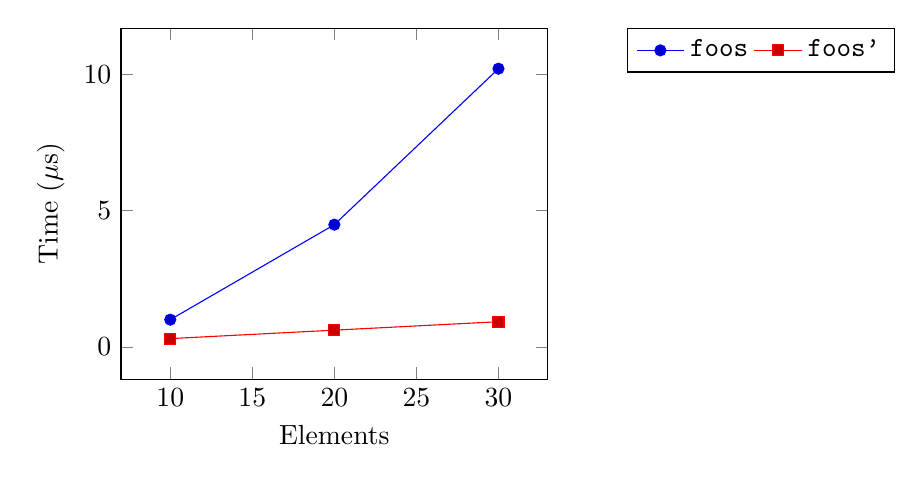
\begin{tikzpicture} \begin{axis}
	[
	    legend style={at={(1.5,1)},
	    	anchor=north,legend columns=-1},
		enlargelimits=0.15,
		ylabel=Time ($\mu$s),
		xlabel=Elements
	]
	\addplot+ [
	sharp plot,
	] coordinates {(10,0.994) (20,4.48)
		(30,10.2)};
	\addplot+ [
	sharp plot,
	] coordinates {(10,0.300) (20,0.610) 
		(30,0.919)};
	\legend{\texttt{foos},\texttt{foos'}}
	\end{axis}
	\end{tikzpicture}
\end{center}
\end{fancyfig}

\taskLine

\subsubsection{Induction on natural numbers}

Recall that we have already proved the following (monoidal) properties about natural numbers in the lecture on equational reasoning:
\begin{displaymath}
\begin{array}{lcrcl}
	\textbf{Left unit} &\qquad & \mathit{add}~Z~x & = & x \\
	\textbf{Right unit} &\qquad & \mathit{add}~x~Z & = & x \\
	\textbf{Associativity} & \qquad & \mathit{add}~x~(\mathit{add}~y~z) & = & \mathit{add}~(\mathit{add}~x~y)~z 
\end{array}
\end{displaymath}

\taskLine

\task[task:succ-comm]{Prove the following property about addition just by rewriting one side of the equation until you end up with the other side:
\begin{displaymath}
\forall n :: \mathit{Nat} . S~n = \mathit{add}~(S~Z)~n
\end{displaymath}
You should show each step of the proof along with a comment to say what you have done at that particular step, as shown in the lecture and the proofs in \Cref{sec:lecture-10}.
}

\task[task:successor-commutes]{Prove the following property about addition by induction on $n$. For this proof, you will need to make use of some of the other properties you know about $\mathit{add}$, including the one you proved for Exercise \ref{task:succ-comm}.
\begin{displaymath}
\forall n~m :: \mathit{Nat} . \mathit{add}~(S~n)~m = \mathit{add}~n~(S~m)
\end{displaymath}
}

\task[task:add-commutes]{Finally, using all the properties you know about $\mathit{add}$ so far, prove that $\mathit{add}$ commutes:
\begin{displaymath}
\forall n~m :: \mathit{Nat} . \mathit{add}~n~m = \mathit{add}~m~n
\end{displaymath}
}

\taskLine

\subsubsection{Induction on lists}

In Haskell, the \haskellIn{reverse} function can be defined as follows:
\begin{minted}{haskell}
reverse :: [a] -> [a]
reverse []     = []
reverse (x:xs) = reverse xs ++ [x]
\end{minted}
This makes use of the \haskellIn{(++)} operator, which is defined as follows:
\begin{minted}{haskell}
(++) :: [a] -> [a] -> [a]
[]     ++ ys = ys 
(x:xs) ++ ys = x : (xs ++ ys)
\end{minted}

\taskLine

\task[task:reverse-identity-left]{Prove that $(\append)$ has a left identity by rewriting the following equation:
\begin{displaymath}
\forall \mathit{xs} :: \hslist{a}~. \quad \hslist{} \append \mathit{xs} = \mathit{xs}
\end{displaymath}}

\task[task:reverse-identity-right]{Prove that $(\append)$ has a right identity by induction on $\mathit{xs}$:
\begin{displaymath}
\forall \mathit{xs} :: \hslist{a}~. \quad \mathit{xs} \append \hslist{} = \mathit{xs}
\end{displaymath}}

\task[task:append-assoc]{Prove that $(\append)$ is associative by induction on $\mathit{xs}$:
	\begin{displaymath}
	\forall \mathit{xs}~\mathit{ys}~\mathit{zs} :: \hslist{a}~. \quad \mathit{xs} \append (\mathit{ys} \append \mathit{zs}) = (\mathit{xs} \append \mathit{ys}) \append \mathit{zs}
	\end{displaymath}}

\task[task:reverse-preserves]{Prove that $\mathit{reverse}$ preserves singleton lists by rewriting the following equation:
\begin{displaymath}
\forall \mathit{x} :: a~. \quad \mathit{reverse}~\hslist{x} = \hslist{x}
\end{displaymath}}

\task[task:reverse-distributes-over-append]{Prove that $\mathit{reverse}$ distributes over $(\append)$ by induction on $\mathit{xs}$. You will need some of the properties you have proved so far about $(\append)$ and $\mathit{reverse}$.
\begin{displaymath}
\forall \mathit{xs}~\mathit{ys} :: \hslist{a}~. \quad \mathit{reverse}~(\mathit{xs} \append \mathit{ys}) = \mathit{reverse}~\mathit{ys} \append \mathit{reverse}~\mathit{xs}
\end{displaymath}}

\task[task:reverse-of-reverse]{Prove the following property about $\mathit{reverse}$ by induction on $\mathit{xs}$. You will need some of the properties you have proved so far about $(\append)$ and $\mathit{reverse}$.
\begin{displaymath}
\forall \mathit{xs} :: \hslist{a}~. \quad \mathit{reverse}~(\mathit{reverse}~\mathit{xs}) = \mathit{xs}
\end{displaymath}}

\taskLine

\subsubsection{Constructive induction}

It is possible to use induction to \emph{calculate} faster function definitions. This is referred to as \emph{constructive induction}. For example, consider our current definition of \haskellIn{reverse}:
\begin{minted}{haskell}
reverse :: [a] -> [a]
reverse []     = []
reverse (x:xs) = reverse xs ++ [x]
\end{minted}
This definition is inefficient because the \haskellIn{(++)} operator runs in $\mathcal{O}(n)$ time where $n$ is the length of the first argument. The \haskellIn{reverse} function runs in quadratic time as a result. We can do better by combining the behaviour of \haskellIn{reverse} and \haskellIn{(++)} into one new function which does both. We begin by expressing this idea as the following specification:
\begin{minted}{haskell}
rev :: [a] -> [a] -> [a]
rev xs ys = reverse xs ++ ys
\end{minted}
The \haskellIn{rev} function takes two lists as arguments, reverses the first and then appends the second list to it. Our goal is now to use induction to come up with a new definition for \haskellIn{rev} which neither uses \haskellIn{reverse} nor \haskellIn{(++)}. We do this by taking the current definition and performing induction on \texttt{\small xs}. Recall that there are two cases for induction on lists: the empty list (a base case) and cons (a recursive case). We can write down a skeleton for the new definition of \haskellIn{rev} by covering these two cases:
\begin{minted}{haskell}
rev :: [a] -> [a] -> [a]
rev []     ys = ???
rev (x:xs) ys = ???
\end{minted} 

\task[task:rev-empty]{Replace the \texttt{\small ???} in the first equation by reducing \haskellIn{reverse [] ++ ys} as much as possible. The resulting expression should neither contain \haskellIn{reverse} nor \haskellIn{(++)}. \emph{Hint}: you only need to apply \haskellIn{reverse} and \haskellIn{(++)} until you are left with an expression which cannot be reduced any further. This expression can then be used as the right-hand side of the first equation above.}

\task[task:rev-cons]{Replace the \texttt{\small ???} in the second equation by reducing \haskellIn{reverse (x:xs) ++ ys} as much as possible. The resulting expression should neither contain \haskellIn{reverse} nor \haskellIn{(++)}. \emph{Hint}: in this case, you can use the specification \texttt{\small rev xs ys = reverse xs ++ ys} as induction hypothesis.}

\taskLine

%\pagebreak

%\begin{center}
%	\vspace*{4cm}
%	\textbf{This page is intentionally left blank.}
%	\vfill
%\end{center}